\documentclass[conference]{IEEEtran}
\IEEEoverridecommandlockouts
\usepackage{listings}
\usepackage{xcolor}
\usepackage{hyperref}
\usepackage{amsthm}
\usepackage{pgfplots}
\usepackage{graphicx}
\graphicspath{ {./time_comp/} }
\lstset { %
    language=C++,
    backgroundcolor=\color{black!5}, % set backgroundcolor
    basicstyle=\footnotesize,% basic font setting
}
%New colors defined below
\definecolor{codegreen}{rgb}{0,0.6,0}
\definecolor{codegray}{rgb}{0.5,0.5,0.5}
\definecolor{codepurple}{rgb}{0.58,0,0.82}
\definecolor{backcolour}{rgb}{0.95,0.95,0.92}

%Code listing style named "mystyle"
\lstdefinestyle{mystyle}{
  backgroundcolor=\color{backcolour},   commentstyle=\color{codegreen},
  keywordstyle=\color{magenta},
  numberstyle=\tiny\color{codegray},
  stringstyle=\color{codepurple},
  basicstyle=\ttfamily\footnotesize,
  breakatwhitespace=false,         
  breaklines=true,                 
  captionpos=b,                    
  keepspaces=true,                 
  numbers=left,                    
  numbersep=5pt,                  
  showspaces=false,                
  showstringspaces=false,
  showtabs=false,                  
  tabsize=2
}

%"mystyle" code listing set
\lstset{style=mystyle}
% The preceding line is only needed to identify funding in the first footnote. If that is unneeded, please comment it out.
\usepackage{cite}
\usepackage{amsmath,amssymb,amsfonts}
\usepackage{algorithmic}
\usepackage{graphicx}
\usepackage{textcomp}
\usepackage{xcolor}
\def\BibTeX{{\rm B\kern-.05em{\sc i\kern-.025em b}\kern-.08em
    T\kern-.1667em\lower.7ex\hbox{E}\kern-.125emX}}
\begin{document}

\title{IIIT Allahabad\\DAA Assignment-06\\
}

\author{\IEEEauthorblockN{Sanket Kokude}
\IEEEauthorblockA{\textit{IIB2019034} \\
}
\and
\IEEEauthorblockN{Harshit Kumar}
\IEEEauthorblockA{\textit{IIB2019035} \\
}
\and
\IEEEauthorblockN{Viful Nirala}
\IEEEauthorblockA{\textit{IIB2019036} \\
}
}

\maketitle

\begin{abstract}
In this report we design a parallel algorithm for the Tower of Hanoi problem where parallel moves are allowed.

\end{abstract}

\section{Introduction}
Tower of Hanoi is a mathematical puzzle where we have three rods and n disks. The objective of the puzzle is to move the entire stack to another rod, obeying the following simple rules: 

\begin{itemize}
\item Only one disk can be moved at a time.
\item Each move consists of taking the upper disk from one of the stacks and placing it on top of another stack i.e. a disk can only be moved if it is the uppermost disk on a stack.
\item No disk may be placed on top of a smaller disk.\\
\end{itemize}

A parallel algorithm is an algorithm that can solve several sub-problem simultaneously and then combine all the individual outputs to produce the final result.

\section{Algorithm Design.1}
Following is the recursive algorithm for TOH:
\begin{itemize}
    \item Move n-1 disks from source to aux.
    \item Move nth disk from source to dest.
    \item Move n-1 disks from aux to dest.
\end{itemize}
\section{Algorithm Design.2}
Following is parallel algorithm :

\begin{itemize}
\item Let number of disks is n, we call the function named $func(0,n-1)$ where $start=0$ and $end=n-1$.
\item First calculate $n$ as $n=end-start+1$.
\item In the function $func$ we first check the number of disks, given by the user whether it is smaller than 2 or not, if it is we call the $toh$ function to move the disk from A to B.
\item If n is greater than $2$ and n is odd, and then we recursively call as $b1=func(start,(start+end)/2-1)$ and $b2=func((start+end)/2,end)$.
 Or if $n$ is greater than $2$ and $n$ is even, and then we recursively call as $b1=func(start,(start+end)/2)$ and $b2=func((start+end)/2+1,end)$.
\item If $n$ is greater than $2$ so we recursively call $func$ again and divide the array into 2 subarrays of size $n/2$ and $n-n/2$ respectively. 
\item We repeat this dividing process until the size of each subarray is less than or equal to 2.
\item If the size of the subarray less than or equal to 2 we call the $toh$ function to arrange the discs into the final tower using the auxiliary tower.
\item The result from all of the $toh$ functions will be stored in arrays named $b1,b2$.
\item After that all of the B arrays are merged together and the final array formed is given as output.\\
\end{itemize}

\section{Algorithm and illustration}
Suppose the given number of disks is 50, then we call the function named func.
\begin{itemize}
\item In the function func we first check the number of disks given by the user. Since 50 is greater than 2 so we recursively call func again and divide the array into 2 subarrays of size n/2 and n-n/2 respectively. 
\item In this case after first recursive calling the formed subarrays will be of size 25 each.
The two formed subarrays are A1[25] which contain the discs 1 to 25 and A2[25] with discs numbered 26 to 50.
\item In case of A1[25], it would again be divided into subarrays containing discs numbered 1 to 12 and 13 to 25.
Similarly for A2[25], It would be divided into subarrays containing discs numbered 26 to 37 and 38 to 50.
\item We repeat this dividing process until the size of each subarray is less than or equal to 2.
\item If the size of the subarray less than or equal to 2 we call the TOH function to arrange the discs into the final tower using the auxiliary tower.
The result from all of the TOH functions will be stored in arrays named B1,B2.
\item In case of 50 discs the total number of B arrays formed is 32.
\item After that all of the B arrays are merged together and the final array formed is given as output.\\
\end{itemize}

\section{Algorithm Analysis}
\textbf{Time complexity:}\\
For recursive algorithm: 
$T(n)=2T(n-1)+1$\\
So the time complexity is $O(2^n)$.\\\\
For parallel algorithm:\\
$T(n) = 2T(n/2) + O(n)$\\
By solving this recurrence relation by master theorem we get time complexity as $O(nlogn)$.\\

\\
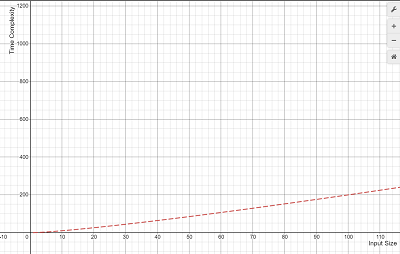
\includegraphics{time_comp}\\\\
\textbf{Space complexity:}\\
For recursive algorithm: space complexity is $O(n)$.\\
For parallel algorithm:\\
In this  approach we will have the space complexity as $O(n)$\\\\
\\\\


\section{Conclusion}
By recursion algorithm the time complexity will be $O(2^n)$ which will be very large to solve for n greater then 15.
Therefore we need parallel algorithm to solve the problem for larger n.
 \section{References}
\color{blue}1.{\url{https://en.wikipedia.org/wiki/Tower_of_Hanoi} }\\
2.{\url{https://www.geeksforgeeks.org/c-program-for-tower-of-hanoi}}\\
3. Cormen, Leiserson, Rivest, and Stein (2009). Introduction to Algorithms, 3rd edition.

\color{black}
\
\begin{titlepage}
    \begin{center}
        \Huge
        \section*{Appendix}
        \end{center}
         \textbf{Code for implementation of this paper is given below:}
\begin{lstlisting}[language=C++,caption=Code for this paper]
#include <bits/stdc++.h>
using namespace std;
struct a{
    int b[1000];
};
int a[1000];
int num=0;

struct a toh(int start,int end){
    struct a brod;
    int btop=0;
    if(start==end){
        brod.b[btop] = a[start];
        a[start]=0;
    }
    else{
        int crod=a[end];
        a[end]=0;
        brod.b[btop++]=a[start];
        a[start]=0;
        brod.b[btop]=crod;
        crod=0;
    }
    return brod;
}

struct a func(int start,int end){
    int n = end-start+1;
    //base
    if(n<=2){
        struct a bb = toh(start,end);
        return bb;
    }
    struct a b1,b2;
    //recursive
    int k=n%2;
    b1=func(start,(start+end)/2-k);
    b2=func((start+end)/2-k+1,end);
    //merge
    struct a arr;
    std::copy(b1.b, b1.b + n/2, arr.b);
    std::copy(b2.b, b2.b + n-n/2, arr.b + n/2);
    return arr;
}

int main(){
    cout<<"Enter the number of disks: ";
    cin>>num;
    for(int i=0;i<num;i++)
        a[i]=i+1;
    struct a bfinal;
    bfinal=func(0,num-1);
    for(int i=0;i<num;i++){
        cout << bfinal.b[i] << endl;
    }
    return 0;
}
   
\end{lstlisting}
\end{titlepage}
\end{document}
